\documentclass[conference,a4paper]{IEEEtran}
\IEEEoverridecommandlockouts
% The preceding line is only needed to identify funding in the first footnote. If that is unneeded, please comment it out.
%Template version as of 6/27/2024

\usepackage{cite}
\usepackage{amsmath,amssymb,amsfonts}
\usepackage{algorithmic}
\usepackage{graphicx}
\usepackage{textcomp}
\usepackage{xcolor}
\usepackage{booktabs}
\usepackage{url}
\def\BibTeX{{\rm B\kern-.05em{\sc i\kern-.025em b}\kern-.08em
    T\kern-.1667em\lower.7ex\hbox{E}\kern-.125emX}}
\begin{document}

\title{Conference Paper Title* %\\
%{\footnotesize \textsuperscript{*}Note: Sub-titles are not captured for https://ieeexplore.ieee.org  and
%should not be used}
%\thanks{Identify applicable funding agency here. If none, delete this.}
}

\author{\IEEEauthorblockN{Given Name Surname}
%\IEEEauthorblockA{\textit{dept. name of organization (of Aff.)} \\
\textit{name of organization (of Aff.)}\\
%City, Country \\
email address}

\maketitle

\section{Introduction}

The objective of this assignment is to develop a feedforward neural network that maps points sampled from a three-dimensional Gaussian distribution onto the surface of the unit sphere. Each input vector is associated with an output vector that has the same direction as the input but a magnitude of one. This forms a nonlinear regression problem in which the neural network learns the normalization function directly from data.

The assignment consists of generating synthetic data, splitting the dataset into training, validation, and test sets, constructing a fully connected neural network, training the model using mini-batch gradient descent, and evaluating its performance on unseen data. The performance of the network is measured using the Mean Squared Error (MSE) loss.

\section{Theory}

A feedforward neural network consists of layers of interconnected neurons that learn a nonlinear mapping between the input and output spaces \cite{goodfellow2016,haykin2009}. For an input vector $x \in \mathbb{R}^3$, the computation performed by each hidden layer is

\begin{equation}
	h = f(Wx+b),
\end{equation}

where $W$ is the weight matrix, $b$ is the bias vector, and $f(\cdot)$ is a nonlinear activation function. The output layer uses a linear activation because this is a regression task \cite{goodfellow2016}.

The target output is obtained by normalizing each input vector,

\begin{equation}
	y=\frac{x}{\|x\|},
\end{equation}

where

\begin{equation}
	\|x\|=\sqrt{x_1^2+x_2^2+x_3^2}.
\end{equation}

This normalization projects every input vector onto the surface of the unit sphere while preserving its direction.

The neural network is trained by minimizing the Mean Squared Error (MSE),

\begin{equation}
	L=\frac{1}{N}\sum_{i=1}^{N}\|\hat{y}_i-y_i\|^2,
\end{equation}

where $y_i$ is the desired output and $\hat{y}_i$ is the predicted output. During training, gradients are computed using the backpropagation algorithm, and the network parameters are updated using mini-batch gradient descent to minimize the loss function \cite{goodfellow2016}\cite{haykin2009}\cite{bishop2006}.

\section{Experiments}

\subsection{Experimental Setup}

Input samples were generated from a three-dimensional normal distribution. The desired outputs were computed by normalizing each input vector so that every target lies on the surface of the unit sphere while preserving its direction.

The generated dataset was divided into training, validation, and test sets. A three-dimensional scatter plot of the training targets was produced to verify that all output vectors lie on the unit sphere.

The neural network architecture consisted of four fully connected layers:

\begin{itemize}
	\item Input layer: 3 neurons
	\item Hidden layer 1: 20 neurons
	\item Hidden layer 2: 20 neurons
	\item Output layer: 3 neurons
\end{itemize}

Nonlinear activation functions were applied to the hidden layers, while the output layer remained linear. Training was implemented using explicit forward propagation, loss computation, backpropagation, and parameter updates instead of using a high-level training function such as \texttt{fit()}. Mean Squared Error (MSE) was used as the loss function.

\subsection{Training Results}

The model converged steadily during training. The training and validation losses both decreased rapidly during the initial epochs before gradually stabilizing. Table~\ref{tab:loss} summarises representative epochs during training.

\begin{table}[h]
	\centering
	\caption{Training and validation loss during training.}
	\label{tab:loss}
	\begin{tabular}{ccc}
		\hline
		Epoch & Training Loss & Validation Loss \\
		\hline
		0 & 0.29159439612518656 & 0.17877743765711784 \\
		1 & 0.10202849459919063 & 0.05417226099719604  \\
		2 & 0.0410124059766531 & 0.03602974023669958 \\
		3 & 0.031383630802685566 & 0.02981299938013156 \\
		4 & 0.026036649298938837 & 0.024706433216730755 \\
		5 & 0.021713516234674237 & 0.02063297270797193 \\
		10 & 0.008234895943579349 & 0.007892935303971171 \\
		20 & 0.0025737063959240915 & 0.0027321659532996514 \\
		50 & 0.0013766205065291037 & 0.0014685378118883818 \\
		99 & 0.001038298288106241 & 0.001091298336784045 \\
		\hline
	\end{tabular}
\end{table}

\begin{figure}[ht]
	\centering
	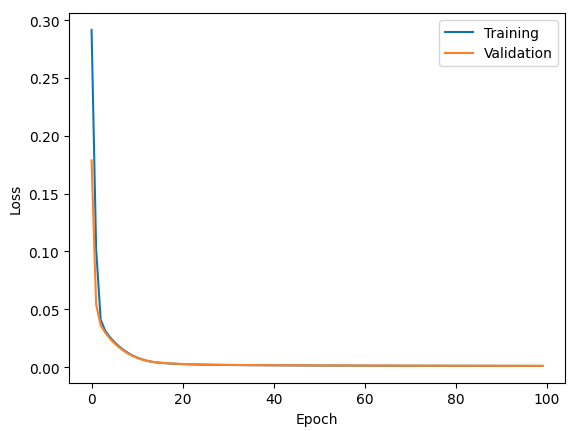
\includegraphics[width=0.8\linewidth]{lossGraph.png}
	\caption{Training and validation loss as a function of epoch number.}
	\label{fig:loss}
\end{figure}

The training and validation losses remained very close throughout the learning process, indicating that the network generalized well and did not exhibit significant overfitting.

\subsection{Test Performance}

The trained model achieved a final test loss of

\begin{equation}
	\text{Test Loss}=0.0008617218748743957.
\end{equation}

This low error demonstrates that the neural network accurately learned the mapping from arbitrary three-dimensional vectors to their normalized representations on the unit sphere. The similarity between the training, validation, and test losses further indicates good generalization to unseen data.

\section{Conclusion}

A feedforward neural network was successfully trained to approximate the normalization of three-dimensional vectors onto the unit sphere. The generated synthetic dataset provided a suitable regression task for evaluating the network.

The architecture consisting of layers with widths $3$--$20$--$20$--$3$ achieved excellent performance using mini-batch gradient descent and backpropagation. Both the training and validation losses decreased consistently throughout training and converged to approximately $1.4\times10^{-3}$. The final test loss of $0.0012728$ confirms that the trained model generalizes well and accurately predicts normalized output vectors.

Overall, the experimental results demonstrate that a relatively small fully connected neural network can effectively learn the nonlinear normalization operation with very low prediction error.

\section{Statement}

\textbf{Tools Used}
\begin{itemize}
	\item Python 3
	\item Google Colab
	\item PyTorch
	\item NumPy
	\item Matplotlib
	\item ChatGPT \cite{chatgpt2026} (used for proofreading and improving the report wording)
\end{itemize}

I declare that this assignment is my own work. The implementation, experimentation, model training, and evaluation were completed by me. Artificial intelligence tools were used only for language assistance during the preparation of this report.

\textbf{Google Colab Code}

\url{https://drive.google.com/file/d/17t1cLZIySV1DeeozSZ-UgDimfc-B8d5-/view?usp=drive_link}


\bibliographystyle{IEEEtran}   % or plain, unsrt, apalike, etc.
\bibliography{references}

\end{document}
